\documentclass[a4paper, 12pt]{article} % Тип документа

%%% Кодировки и локализация
\usepackage[T2A]{fontenc}        % Поддержка кириллицы
\usepackage[utf8]{inputenc}      % Кодировка исходного текста
\usepackage[english, russian]{babel} % Локализация и переносы

%%% Основные настройки документа
\usepackage[a4paper, left=1.5cm, right=1.5cm, top=2.5cm, bottom=2.5cm]{geometry} % Поля страницы
\setlength{\parindent}{1.25cm}   % Размер абзацного отступа
\setlength{\parskip}{0.5em}      % Интервал между абзацами
\usepackage{indentfirst}         % Отступ у первого абзаца

%%% Математические пакеты
\usepackage{amsmath, amsfonts, amssymb, mathtools} % Формулы и символы

%%% Работа с графикой
\usepackage{graphicx}            % Вставка изображений
\usepackage{float}               % Плавающие объекты (рисунки, таблицы)
\usepackage{tikz}                % Рисование схем и графиков
\usepackage{circuitikz}          % Рисование электрических схем

%%% Таблицы
\usepackage{multirow}            % Объединение строк в таблицах
\usepackage{booktabs}            % Улучшенные таблицы

%%% Настройка заголовков
\usepackage{titlesec}
\titleformat{\section}
  [block] % Оформление секции как блока
  {\centering\Large\bfseries} % Выравнивание по центру, шрифт полужирный и увеличенный
  {} % Номер секции (пусто для отключения)
  {0pt} % Отступ между номером и заголовком
  {} % Дополнительное форматирование

%%% Цвета и гиперссылки
\usepackage{xcolor}              % Работа с цветами
\usepackage{hyperref}            % Ссылки в документе
\hypersetup{
    colorlinks=true,
    linkcolor=blue,
    filecolor=magenta,
    urlcolor=blue
}

% Макрос для вставки изображений
\newcommand{\insertimage}[4][0.5]{
    \begin{figure}[H]
        \centering
        \includegraphics[width=#1\linewidth]{#2}
        \caption{\centering #3}
        \label{fig:#4}
    \end{figure}
}

%%% Работа с PDF
\usepackage{pdfpages} % Вставка PDF-страниц в документ


\title{{Отчёт о выполнении работы 3.7.1}\\
       \textbf{Скин-эффект}}
\author{Александр Лобачев}
\date{Сентябрь 2024}

\begin{document}

\begin{titlepage}
    \centering
    \vspace*{\fill}
    {\Huge{Отчёт о выполнении работы 3.7.1}}\\[1cm]
    {\LARGE \textbf{Скин-эффект}}\\[2cm]
    \vfill
    {\Large Александр Лобачев}\\[0.5cm]
    {\Large Ноябрь 2024}
    \vspace*{\fill}
\end{titlepage}


\tableofcontents
\newpage

\textbf{Цель работы}: исследование проникновения переменного магнитного поля в медный полый цилиндр 

\textbf{В работе используются}: генератор сигналов АКИП–3420, соленоид, намотанный на полый
цилиндрический каркас, медный экран в виде полого цилиндра, измерительная катушка, амперметр, вольтметр, двухканальный осциллограф GOS–620, RLC-метр.

 Амплитуда переменного электрического поля с частотой убывает вглубь проводника по экспоненциальному закону. Такой закон спадания характеризуется расстоянием , на котором амплитуда поля уменьшается в $e$ раз. Это расстояние
 называют глубиной проникновения поля или \textit{скиновой} длиной. Явление, при котором амплитуда электромагнитной волны уменьшается при проникновении вглубь проводника, называется \textit{скин-эффектом}

\section{Теоретические сведения}
 
\subsection{Квазистационарное приближение, уравнение диффузии поля}
Если характерная частота изменения электромагнитного поля достаточно мала по сравнению с проводимостью среды, то в уравнении Максвелла в системе СИ:

\[
\oint_{l} \mathbf{H} \cdot d\mathbf{l} = \int_S \mathbf{j} \cdot d\mathbf{S} + \int_S \frac{\partial \mathbf{D}}{\partial t} \cdot d\mathbf{S}
\]

можно пренебречь вторым слагаемым и воспользоваться в дифференциальной форме законом Ома ($\sigma$ - проводимость среды), тогда
\begin{equation}
   \text{rot} \, \mathbf{H} = \sigma \mathbf{E} 
   \label{Amper}
\end{equation}

Это приближение соответствует бесконечной скорости распространения волн вне проводника. Такое приближение называется \textit{квазистационарным}. Более строго, характерные размеры системы должны быть меньше длины волны и плотность тока смещения должна быть меньше плотности тока проводимости:

\begin{equation}
    \nu << \frac{c}{a}, \text{   } \nu << \frac{\sigma}{\varepsilon \varepsilon_0}
    \label{boundary conditions}
\end{equation}

И для меди $\sigma \approx 6 \cdot 10^7 \text{ См/м}$ выполняется, в целом, с запасом. Если мы используем закон Ома в таком виде, то частота колебаний поля должна быть меньше частоты столкновений электронов с решёткой.

Возьмём ротор от обеих частей уравнения (\ref{Amper}), тогда

\[\text{rot} \text{rot} \, \mathbf{H} = \sigma \text{rot} \mathbf{E} = \text{grad div} \mathbf{H} - \nabla^2 \mathbf{H} \]

Согласно 2 уравнению Максвелла, магнитных зарядов не существует и дивергенция $B$ = 0, а ротор $E$ выразим через закон электромагнитной индукции. Пользуемся материальными уравнениями $\mathbf{B} = \mu \mu_0 \mathbf{H}$

\[ \text{div} \mathbf{B} = 0 \]

\begin{equation}
    \text{rot} \mathbf{E} = - \frac{\partial \mathbf{B}}{\partial t}
    \label{electromagnetic induction}
\end{equation} 

Откуда получаем уравнение, аналогичное явлениям переноса (диффузия, теплопроводность)


\begin{equation}
    \nabla^2 \mathbf{H} = \sigma \mu \mu_0 \frac{\partial \mathbf{H}}{\partial t}
    \label{the diffusion equation}
\end{equation}

Для напряжённости электрического поля можно записать аналогичное уравнение, в котором роль коэффициента диффузии играет

\[D_\text{э/м} = \frac{1}{\sigma \mu \mu_0} \approx 130 \text{ см}^2 / \text{с}\]

Тогда согласно закону Эйнштейна-Смолуховского можно оценить среднее расстояние \textit{проникновения поля вглубь проводника} (аналогично задаче о выравнивании температур или концентраций различных газов в модели случайных блужданий).

\[<\Delta r^2> = 2 D_\text{э/м} t\]

Тогда \textit{скиновая глубина} в поверхностном случае в одномерном случае

\begin{equation}
    \delta = \sqrt{2D_\text{э/м} t} = \sqrt{\frac{2}{\sigma \mu \mu_0} t}
    \label{the depth of the skin layer}
\end{equation}

\begin{enumerate}
    \item $\nu = 50 \text{ Гц}$: $\delta \sim 1,5 \text{ см}$
    \item $\nu = 50 \text{ кГц}$: $\delta \sim 0,5 \text{ мм}$
\end{enumerate}

Можно оценить характерное время проникновения тока вглубь проводника как диффузионное приближение для медного провода толщиной 0,5 мм:

\[ \tau \sim \frac{r^2}{D_\text{э/м}} \approx 2 \cdot 10^{-5} \text{ с}\]


\subsection{Модель полубесконечного цилиндра}
Рассмотрим скин-эффект в полубесконечном пространстве. При выполнении условий (\ref{boundary conditions}) можно пренебречь краевыми эффектами и положить, что поле $\mathbf{H}$ направлено вдоль оси $Z$, а вихревое электрическое поле $E$ направлено по концентрическим окружностям в плоскости, перпендикулярной боковой поверхности.

 Простейшим частным решением \textit{волнового уравнения} в безграничном пространстве является плоская волна:
 \[E(t, r) = E_0 \sin{(\omega t - \mathbf{k} \cdot r)} \]

 Тогда можно воспользоваться \textit{методом комплексных амплитуд} и представить амплитуду компонент $\mathbf{E} \text{ и } \mathbf{H}$ в виде

 \begin{equation}
     H_z = H(r) e^{i \omega t}, \text{    } E_\varphi = E(r) e^{i \omega t} 
 \end{equation}

\begin{figure}[h!]
    \centering
    \begin{tikzpicture}[scale=1.6]

    % Радиус цилиндра (a) и толщина стенок (h)
    \def\a{1.5} % радиус цилиндра
    \def\h{0.3} % толщина стенки
    \def\angle{-30} % угол наклона образующих (в градусах)

    % ===== Передние круги =====
    % Закрашивание серых стенок
    \fill[gray!30] (0,0) circle (\a+\h); % внешний круг
    \fill[white] (0,0) circle (\a); % внутренний круг (белый, не закрашенный)

    % Границы кругов
    \draw[thick] (0,0) circle (\a+\h); % граница внешнего радиуса
    \draw[thick] (0,0) circle (\a); % граница внутреннего радиуса
    \draw[dashed, thick] (0,0) circle (0.4 * \a); % циркуляция

    % ===== Образующие цилиндра =====
    % Сплошные образующие
    \draw[thick] ({-\a+1.23 * \h}, \a -0.30 * \h) -- ++({2.8*cos(\angle)}, {-2.8*sin(\angle)});
    \draw[thick] ({\a-1.23 * \h}, -\a  + 0.30 * \h) -- ++({3*cos(\angle)}, {-3*sin(\angle)});
    % Пунктирные образующие
    \draw[dashed, thick] ({-\a}, 0) -- ++({3.5*cos(\angle)}, {-3.5*sin(\angle)});
    \draw[dashed, thick] ({\a+\h}, 0) -- ++({2*cos(\angle)}, {-2*sin(\angle)});

    % циркуляция
     % Радиус a
    \draw[->, thick] (-0.4 * \a, 0) arc[start angle=178, end angle=180, radius=\a] node[midway, right] {\(E_\varphi\)};


    % ===== Ось z =====
    \fill (0, 0) circle (1.5pt);  % Заполненная точка с радиусом 2pt
    \draw[dashed, ->, thick] (0,0) -- ++({4*cos(\angle)}, {-4*sin(\angle)}) node[below right] {\(z\)};

    \draw[->, thick] ({3 * cos(\angle)}, {-2 * sin(\angle)}) -- ++({1 * cos(\angle)}, {-1 * sin(\angle)}) node[below right] {\(H_z\)};


    % ===== Обозначения размеров =====
    % Радиус a
   \draw[->, thick] (0,0) -- ++(\a, 0) node[below left] {\(a\)};
    % Толщина стенки h
    \draw[<->] ({\a+\h}, 0) -- (\a, 0) node[midway, below] {\(h\)};

\end{tikzpicture}
 \caption{Распределение полей в тонкостенном медном цилиндре}
    
\end{figure}



В силу граничных условий имеем

\[ \Delta E_\tau = 0, \text{    } \Delta H_\tau = 0\]

Поэтому $\mathbf{E}(r) \text{ и } \mathbf{B} (r)$ непрерывны всюду. При условии, что толщина стенок $h << a$ можно воспользоваться одномерным приближением и рассматривать и рассматривать поле $\mathbf{H}$ внутри однородным вследствие отсутствия токов. Из уравнения (\ref{electromagnetic induction}) можно найти зависимость амплитуды электрического поля от расстояния

\[ E_\varphi \cdot 2\pi r = - \mu_0 \pi r^2 \frac{d H_z}{d t}\]

Используя (\ref{the depth of the skin layer}), получаем следующее соотношение

\[ E(r) = - \frac{1}{2} \mu_0 r \cdot i \omega H_1\]

На внутренней поверхности при $r = a$ имеем 

\begin{equation}
    E_1 = - \frac{1}{2} \mu_0 a i \omega H_1
    \label{function E_1 expession}
\end{equation}

Здесь $H_1$ - амплитуда напряжённости магнитного поля внутри цилиндра. Напомним, она полагается постоянной и не зависящей от $r$.

\subsection{Плоская геометрия скин-эффекта}

\begin{figure}[h!]
    \centering
    \begin{tikzpicture}[scale = 1.5]
    % Рамка
    \fill[gray!30] (0, -2) rectangle (2, 2);

    % Вектора E0 и E1
    \draw[ thick] (0, 0) -- (0, 2) node[midway, left] {$\mathbf{E_0}$};
    \draw[ thick] (2, 0) -- (2, 2) node[midway, right] {$\mathbf{E_1}$};

    % Вектора H0 и H1
    \draw[ thick] (0, 0) -- (0, -2) node[midway, left] {$\mathbf{H_0}$};
    \draw[ thick] (2, 0) -- (2, -2) node[midway, right] {$\mathbf{H_1}$};

    % Оси координат
    \draw[->, thick] (-0.5, 0) -- (2.5, 0) node[below right] {$x$};
    \draw[->] (0, 0) -- (0, -2.9) node[below left] {$y$};
    \node[below left] at (0, 0) {$0$};
    \node[above left] at (0, 0) {$z$};

    % Векторное обозначение
    \node at (-0.3, -1.7) {$\otimes$};
    \node at (2.3, -1.7) {$\otimes$};
    \node at (-0, 0) {$\otimes$};

    % Обозначения h и a
    \draw[<->] (0, -2.2) -- (2, -2.2) node[midway, below] {$h$};
    \draw[->]  (3.2, 0.3) -- (2, 0.3) node[midway, above] {$a$};

\end{tikzpicture}
\caption{Поле в стенке цилиндра} 
\label{electromagnetic field}
\end{figure}


Мы выяснили, что $\mathbf{H}$ направлен вдоль оси $Z$, поэтому $H_x = H_y = 0$ и $H_z = H_z (x, t)$. Перепишем уравнение (\ref{the diffusion equation}) для компоненты поля $\mathbf{E}$ и оно примет вид:

\[ \frac{\partial^2 H_z}{\partial x^2} = \sigma \mu \mu_0 \frac{\partial H_z}{\partial t}\]

Подставляю выражение для $H_z$ из (\ref{the diffusion equation}), имеем

\begin{equation}
    \frac{d^2 H}{d x^2} = i \omega \sigma \mu_0 H
    \label{the equation on H}
\end{equation}

Граничные условия зададим $H(0) = H_0, H(h) = H_1$

Поскольку цилиндр помещён в соленоид, то $H_0$ - внешнее поле цилиндра, равное полю внутри соленоида без цилиндра.

Характеристическое уравнение (\ref{the equation on H}): $\lambda^2 = i \omega \sigma \mu_0$. Получаем два корня $\lambda = \pm \alpha$, где $\alpha = \sqrt{i \omega \sigma \mu_0} = \frac{\sqrt{2}}{\delta} e^{\frac{i \pi}{4}}$. Тогда решение ищем в виде

\[H(x) = A e^{\alpha x} + Be^{-\alpha x}\]

Константы $A$ и $B$ ищутся из граничных условий: $A + B = H_0$

И пользуемся уравнением (\ref{Amper}). После исключения $A$ и дифференцирования получим выражение для $E(x)$:

\[E(x) = \frac{1}{\sigma} \frac{d H}{d x} = \frac{\alpha}{\sigma} (- H_0 e^{\alpha x} + 2B \cosh{\alpha x})\]

После этого можно воспользоваться граничным условием (\ref{function E_1 expession}) и положить $x = h$, после чего можно исключить $B$ и получить связь на $H_1$ и $H_0$:

\begin{equation}
    H_1 = \frac{H_0}{\cosh{\alpha h} + \frac{1}{2} \alpha a \sinh{\alpha h}}
    \label{The relationship between the H_1 and H_0}
\end{equation}

\subsection{Предельные случаи}
\begin{enumerate}
    \item Толщина скин-слоя \textit{превосходит} толщину цилиндра, тогда $|\alpha h| << 1$ и 
    \begin{equation}
        H_1 = \frac{H_0}{1 + i\frac{ah}{\delta^2}}
        \label{frequency response}
    \end{equation}

Вторым слагаемым в знаменателе пренебречь нельзя, так как возможна ситуация, при которой $h << \delta << a$. Мы получили как бы передаточную функцию для компоненты поля $H$, откуда сдвиг фаз $\psi$ определяется равенством:

\begin{equation}
    \tan{\psi} = \frac{a h}{\delta^2}
    \label{low frequencies phase}
\end{equation}

    \item Случай \textit{больших частот}. Толщина скин-слоя становится меньше толщины стенки. Тогда приближение $\sinh$ и $\cosh$ при $|\alpha h| >> 1$ даёт $\frac{e^{\alpha h}}{2}$ и (\ref{The relationship between the H_1 and H_0}) преобразуется к виду:

\begin{equation}
    H_1 = H_0 \frac{4}{\alpha a} e^{- \alpha h} = \frac{2 \sqrt{2} \delta}{a} e^{- \frac{h}{\delta}} e^{-i \left(\frac{\pi}{4} + \frac{h}{\delta}\right)}
\end{equation}

Отсюда сразу видно, что поле в цилиндре меньше в $\frac{2 \sqrt{2} \delta}{a} e^{- \frac{h}{\delta}}$, а сдвиг фаз 

\begin{equation}
    \psi = \frac{\pi}{4} + \frac{h}{\delta} = \frac{\pi}{4} + h\sqrt{\frac{\omega \sigma \mu_0}{2}}
    \label{high frequenncies phase}
\end{equation}

\end{enumerate}

\section{Методика эксперимента}

\subsection{Экспериментальная установка}


\begin{figure}[h!]
    \centering
    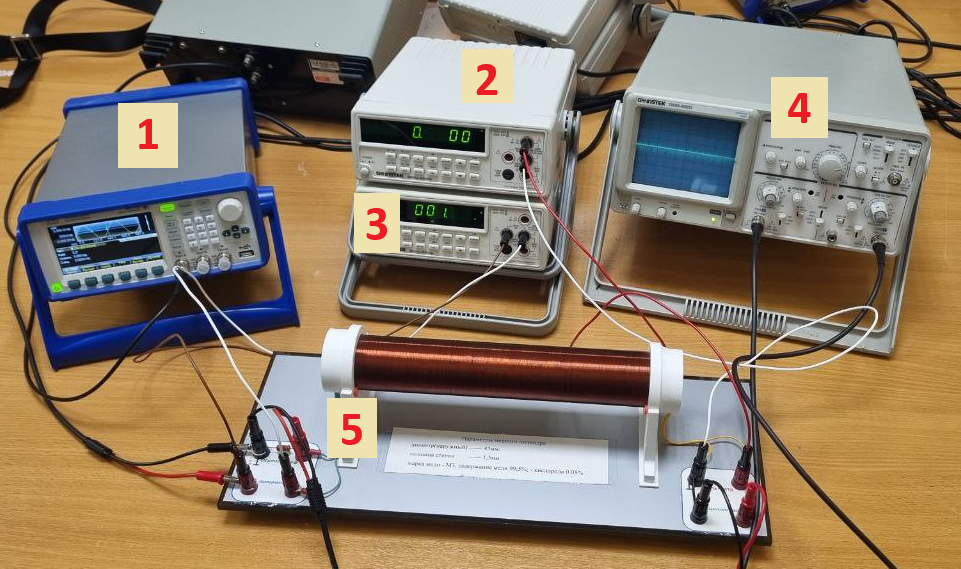
\includegraphics[width=0.75\linewidth]{real installation sheme.png}
    \caption{Экспериментальная установка по изучению скин-эффекта}
    \label{real installation sheme}
\end{figure}

\begin{figure}[h!]
    \centering
    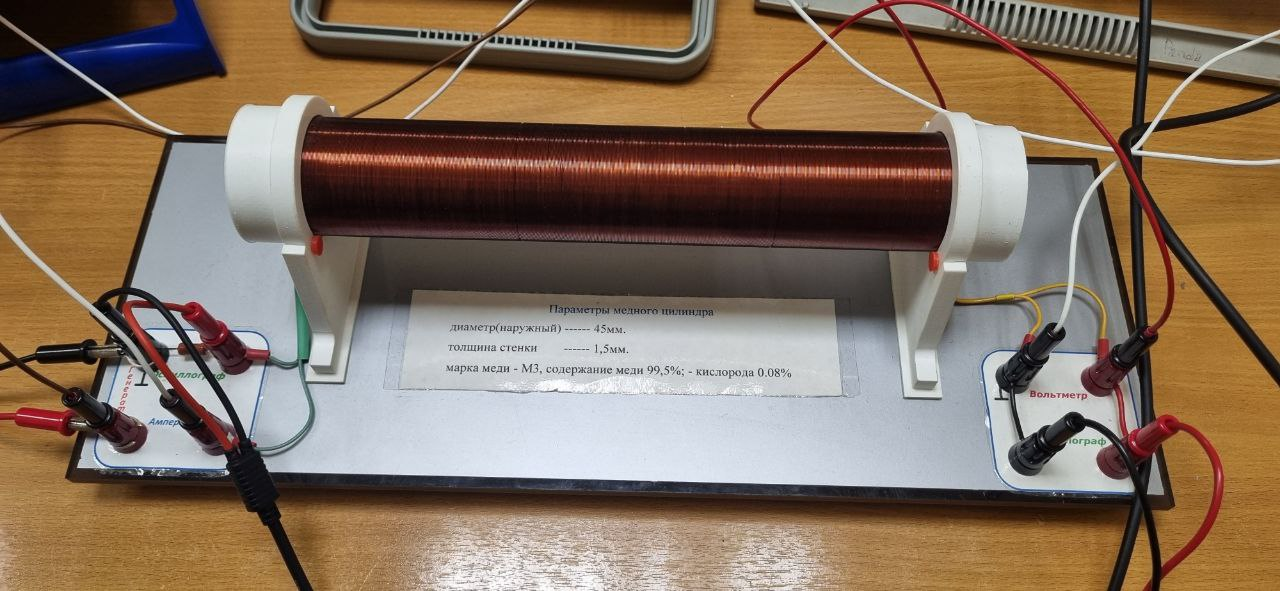
\includegraphics[width=0.75\linewidth]{copper cylinder.jpg}
    \caption{Корпус соленоида с медным цилиндром внутри}
    \label{copper cylinder}
\end{figure}

\begin{figure}[h!]
    \centering
    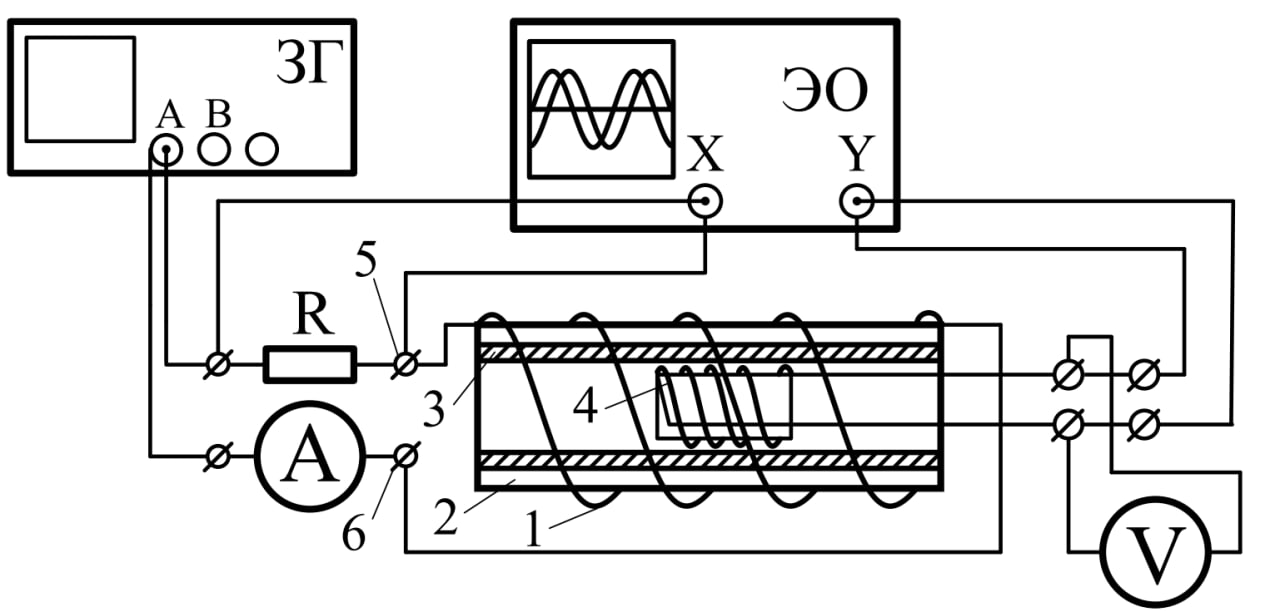
\includegraphics[width=0.75\linewidth]{installation_sheme.jpg}
    \caption{Схема экспериментальной установки}
    \label{installation sheme}
\end{figure}

Соленоид 1 намотан на цилиндрическую трубу из поливинилхлорида, который обладает хорошей диэлектрической проницаемостью и используется для изоляции проводов и кабелей. Внутри расположен медный экран 3 в виде полого цилиндра с параметрами. Действующие значения тока и напряжения измеряются амперметром и вольтметром соответственно. Для измерений сдвига фаз используется осциллограф в двухканальном режиме, так, что канал X подключается к резистору (напряжение в нём пропорционально току через соленоид), а канал Y подключается к измерительной катушке 4. 

На рис (\ref{real installation sheme}): 1 - генератор частот, 2 - вольтметр, 3 - амперметр, 4 - осциллограф, 5 - измерительная установка с исследуемым образцом.

\subsubsection{Инструментальная погрешность измерительных приборов}

\textbf{GDM-8245 в режиме измерения переменного напряжения}:\\ 
± (0,5 \% + 15ед.) на пределе 500мВ/.../500В (45Гц...2кГц) \\
± (1\% + 15ед.) на пределе 500мВ/.../500В (2кГц...10кГц)

\textbf{GDM-8245 в режиме измерения переменного тока}:\\ 
± (0,5 \% + 15ед.) на пределе 500мкА/.../500мА (45Гц...2кГц)
± (1 \% + 15ед.) на пределе 500мкА/.../500мА (2кГц...10кГц)

\textbf{Параметры медного цилиндра}: \\
Диаметр (наружный) ---- 45 мм \\
Толщина стенки ---- 1,5 мм \\
Содержание меди марки М3 в образце ---- 99,5 \%

\subsection{Измерение отношения амплитуд магнитного поля внутри и вне цилиндра}
Поскольку измерительная катушка находится в переменном магнитном поле $H_1 e^{i \omega t}$, возникает ЭДС индукции в катушке 4, действующее значение которой фиксирует вольтметр $V$.

\begin{equation}
    \mathbf{U} = - SN \frac{dB_1}{dt} = - i \omega \mu_0 S N H_1 e^{i \omega t}
    \label{voltmetr, Y channel}
\end{equation}

Тогда вольтметр снимает действительную часть, делённую на $\sqrt{2}$ и можно заключить, что $|H_1| \sim \frac{U}{\omega} \sim \frac{U}{\nu}$

Из теоремы о циркуляции следует, что вне экрана $|H_0|$ пропорциональна току в цепи соленоида, который течёт через амперметр. Отсюда следует:

\begin{equation}
    \frac{|H_1|}{|H_0|} = const \frac{U}{\nu I}
    \label{attenuation coefficient}
\end{equation}

\subsection{Измерение проводимости материала цилиндра}

Измерения будем проводить по фазово-частотной зависимости. Согласно пункту 1.4, для низких частот используем (\ref{low frequencies phase}), для высоких - (\ref{high frequenncies phase}). При больших частотах зависимость $\psi(\sqrt{\nu} \ \frac{\pi}{4})$ аппроксимируется прямой, проходящей через начало координата, аналогично при малых частотах поведение зависимости $\tan{\psi} (\nu)$ тоже является линейной функцией, проходящей через начало координат. При этом, как следует из формулы (\ref{voltmetr, Y channel}), напряжение на измерительной катушке, пропорционально \textit{производной} поля внутри цилиндра. Если занести $i$ в экспоненту, то получим фазовый сдвиг, измеренный по осциллографу:

\begin{equation}
    \phi = \psi + \frac{\pi}{2}
\end{equation}

\newpage

\section{Обработка результатов}

\begin{figure}[h!]
    \centering
    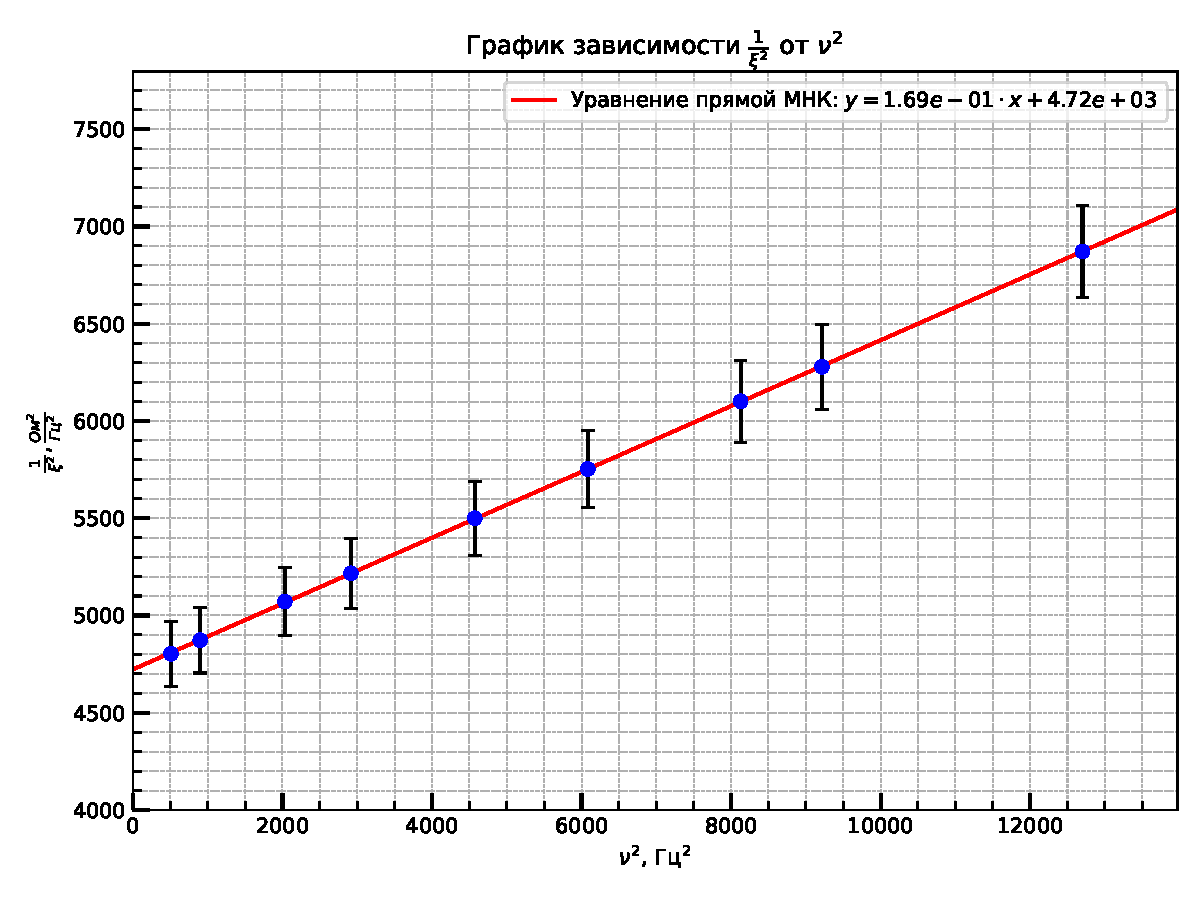
\includegraphics[width=0.95\linewidth]{skin1.pdf}
    \caption{График зависимости $\frac{1}{\xi^2} (\nu^2)$}
    \label{skin 1}
\end{figure}

\subsection{Измерения амплитуд в области низких частот}
	В области низких частот толщина скин-слоя превосходит толщину стенок образца $ \delta \gg h$  и из (\ref{attenuation coefficient}) получаем
    
	\begin{equation*}
		\left(\frac{|H_1|}{|H_0|}\right)^2 = (\xi_0\xi)^2 \approx \frac{1}{1+\left(\frac{ah}{\delta^2}\right)^2} = \frac{1}{1 + \left(\pi ah\nu\mu_0\sigma\right)^2}
	\end{equation*}
    
	Тогда: 
	\begin{equation*}
		\frac{1}{\xi^2}=\xi_0^2 H^2\nu^2 + \xi_0^2 \text{, где } H=\pi a h \sigma \mu_0
		\label{eq:liniya_dlya_c}
	\end{equation*}
    
	По найденным коэффициентам аппроксимации МНК находим: $\xi_0^2 = 4720 \text{ Гц}^2 / \text{Ом}^2$ , тогда:
	\[\xi_0 = 68,7 \pm 0,04 \ \frac{\text{Гц}}{\text{Ом}}, \ \sigma = (5,603 \pm 0,014) \cdot 10^7 \ \frac{\text{См}}{\text{м}}  \]
	
	\subsection{Измерение проводимости через разность фаз при низких частотах}

    \begin{figure}[h!]
    \centering
    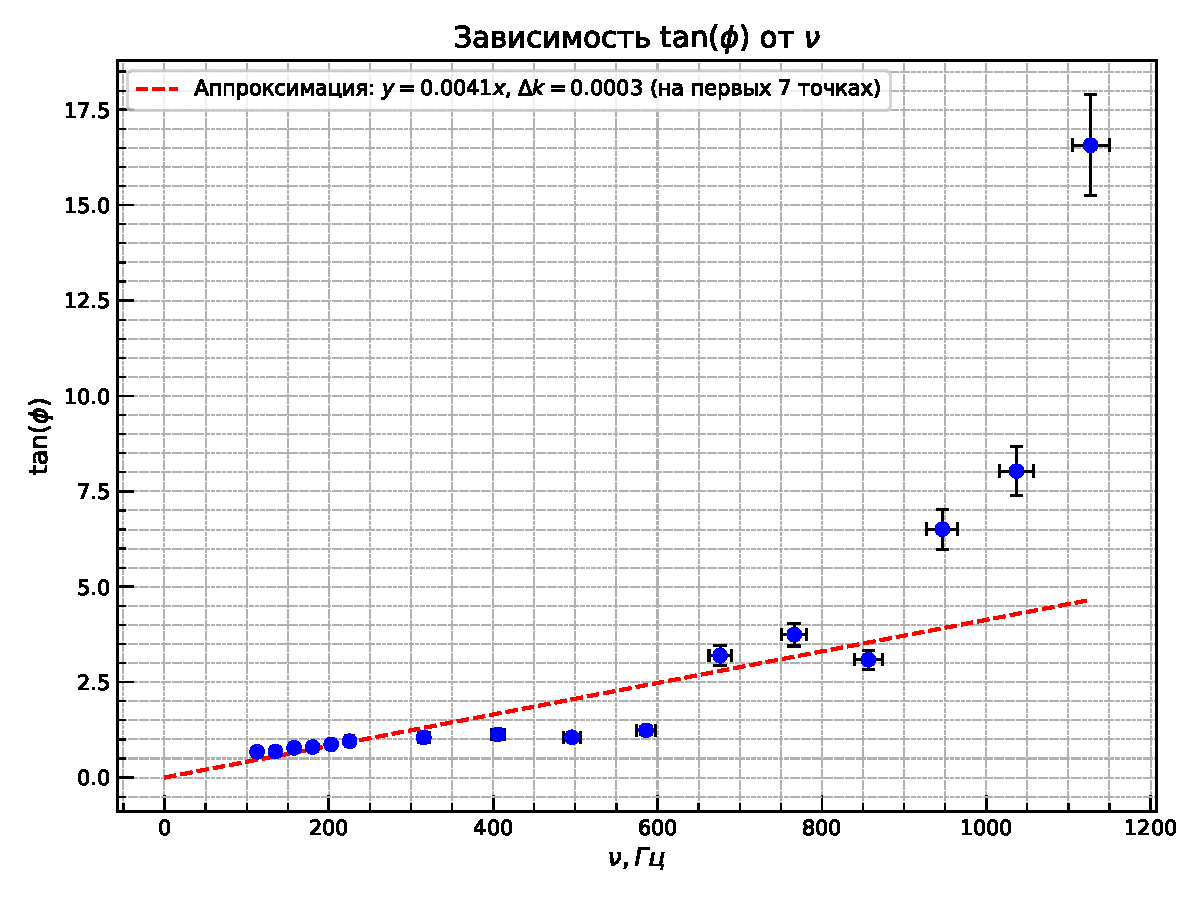
\includegraphics[width=0.95\linewidth]{low frequencies.pdf}
    \caption{График зависимости $\tan{\phi} (\nu)$}
    \label{low frequencies}
    \end{figure}
        
	Построим график $\tg{\psi} (\nu)$ по первым 7 точкам, для которых зависимость хорошо аппроксимируется прямой.
	Согласно формуле (\ref{low frequencies phase}), при $\delta \gg h$
	\begin{equation*}
		\tg \psi = \frac{ahw \sigma \mu_0}{2} = \pi ah\mu_0\sigma \nu \ \
	\end{equation*}
	Коэффициент наклона прямой: \[\pi ah \mu_0\sigma = k = (4,41 \pm 0,13) \cdot 10^{-3} \ \text{с}\]
	\[\sigma = \frac{k}{\pi ah \mu_0} = (3,07 \pm 0,23) \cdot 10^7 \ \frac{\text{См}}{\text{м}}\]

    \newpage

	\subsection{Измерение проводимости через разность фаз в высокочастотном диапазоне}
	Согласно формуле (\ref{high frequenncies phase}), при $\delta \ll h$
	\begin{equation*}
		\psi - \pi/4 = k\cdot \sqrt{\nu}; \ k = h\sqrt{\pi\mu_0\sigma}
	\end{equation*}
	
	Коэффициент наклона прямой $k = 0,0212 \pm 0,0002$, проходящей через начало координат. Отсюда получаем значение проводимости:
	
	\begin{equation}
		\sigma = (5,05 \pm 0,17) \cdot 10^7 \ \frac{\text{См}}{\text{м}}
	\end{equation}
	
	\begin{figure}[h!]
		\centering
		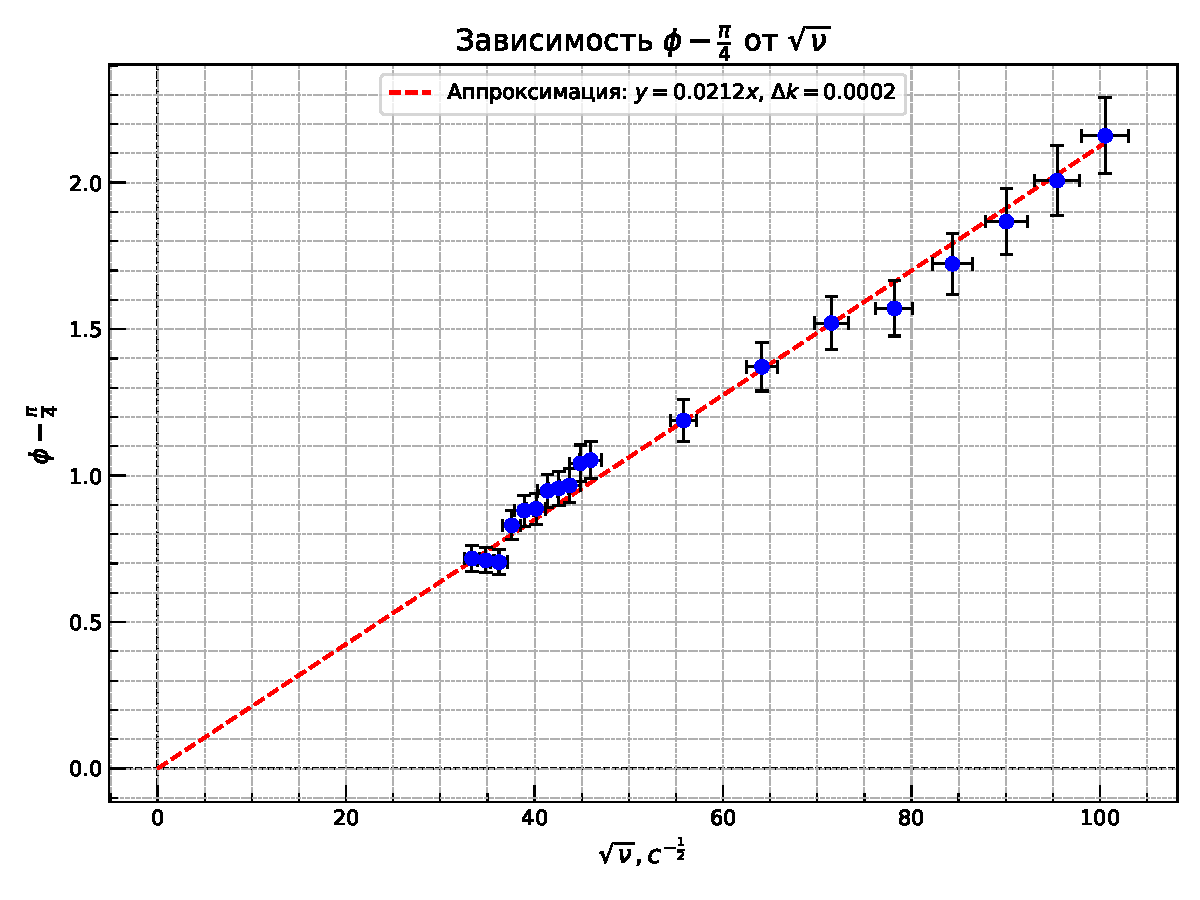
\includegraphics[width=\textwidth]{high frequencies.pdf}
		\caption{График зависимости $(\psi - \pi/4)(\sqrt{\nu})$}
        \label{high frequencies}
	\end{figure}
	
	\subsection{Измерение проводимости через изменение индуктивности}
    \subsubsection{Теоретическая справка}
    
    Поскольку на высоких частотах магнитное поле не проникает внутрь соленоида, то \textit{индуктивность} зависит от \textit{частоты} переменного тока. Суммарный магнитный поток уменьшается из-за уменьшения скиновой глубины, а на низких частот хоть магнитное поле и проникает внутрь экрана, но амплитуда его падает (\ref{frequency response}) и возникает разность фаз колебаний поле внутри и снаружи экрана (\ref{low frequencies phase}). 

    Суммарный магнитный поток, пронизывающий катушку, можно разбить на поток пронизывающий область между катушкой и экраном и область за экраном согласно (\ref{electromagnetic field}).

    \[ \text{Ф} = H_0 S_0 + H_1 S_1 = L I\]

    Индуктивность становится минимальной, когда поле сосредоточено только во внешней области 
    
    \begin{equation}
        L_{min} = \frac{\text{Ф}_\text{внеш}}{I}
        \label{L_min}
    \end{equation}

    Домножим и разделим выражение для внутреннего потока на внешний поток, получим:

    \[\text{Ф}_\text{внутр.} = H_1 S_1 \cdot \frac{\text{Ф}_\text{внеш.}}{H_0 S_0} = \frac{\text{Ф}_\text{внешн.}}{n} \frac{S_1}{S_0}\]

    Из (\ref{attenuation coefficient}) можно выразить $n$ - коэффициент ослабления поля

    Напротив, максимальная индуктивность достигается при равенстве полей $H_1$ и $H_0$. То есть максимальном потоке поля во внутренней области.

    \[ L_{max} = \frac{\text{Ф}_{max}}{I_m}\]

     С учётом (\ref{L_min}) имеем отношение площадей через индуктивности:

     \begin{equation}
         \frac{S_1}{S_0} = \frac{L_{max} - L_{min}}{L_{min}}
     \end{equation}

     Используем (\ref{frequency response}), (\ref{low frequencies phase}), (\ref{the depth of the skin layer}) и связь отношений площадей с отношениями полей и индуктивностей имеем зависимость

     \begin{equation}
         \frac{L_{max} - L}{L - L_{min}} = (\pi a h \mu_0 \sigma)^2 \cdot \nu^2
         \label{L(nu^2)}
     \end{equation}
     
    \subsubsection{Экспериментальная установка}
	Схема экспериментальной установки для нахождения проводимости $\sigma$ по изменению индуктивности катушки $L$ изображена на риc (\ref{LCR installation sheme}). RLC-метр, измеряющий индуктивность, подключается к катушке 1 через клеммы 5 и 6 на панели установки. Другие приборы при этом должны быть отсоединены от цепи, т.к. RLC-метр измеряет индуктивность активным образом. \textbf{Особенность измерений} состоит в том, что прибор даёт ошибочные показания на некоторых частотах, указанных на корпусе (750 Гц, 1 кГц, 5 кГц, 10 кГц)

    \textbf{Инструментальная погрешность RLC-метра ТЕТРОН-RLC200}: 0,1 \% на всех используемых частотах измерений


    \begin{figure}[h!]
		\centering
		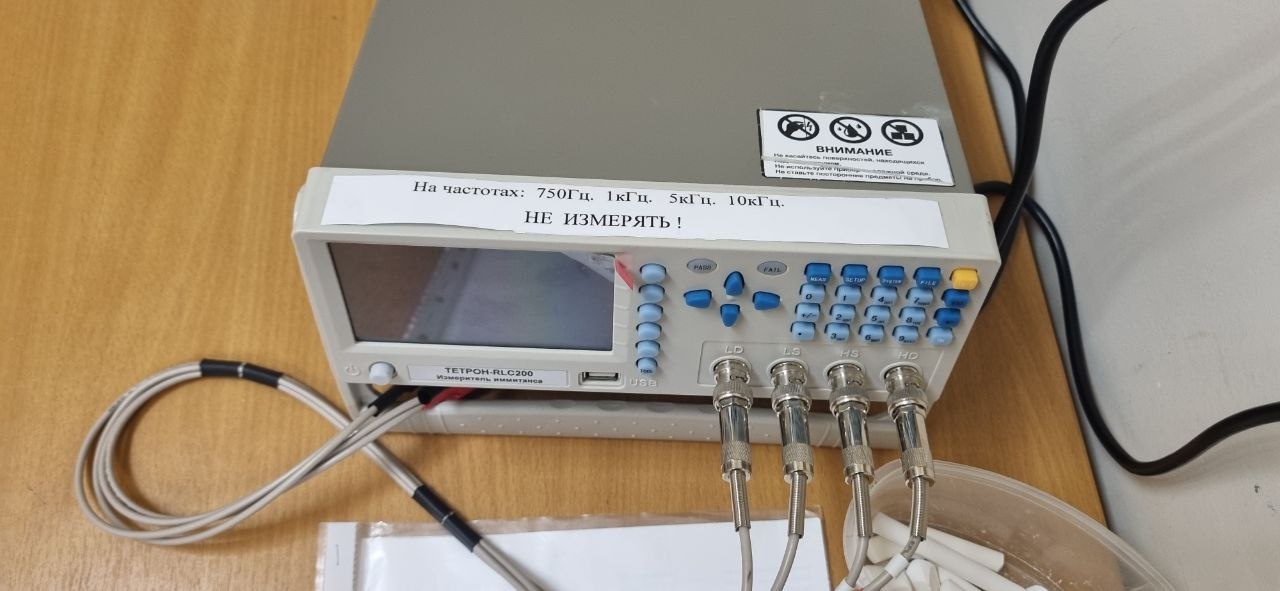
\includegraphics[width=\textwidth]{LCR-metr.jpg}
		\caption{RLC-метр ТЕТРОН-RLC200}
        \label{LCR-metr}
	\end{figure}

    \begin{figure}[h!]
		\centering
		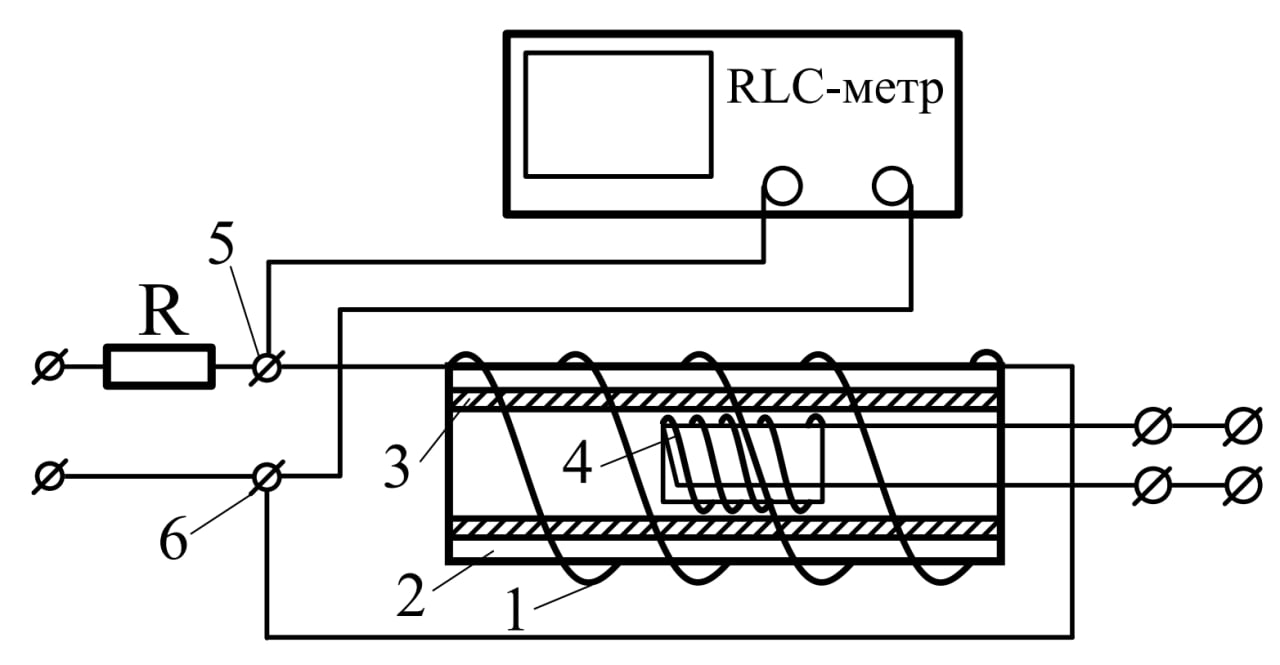
\includegraphics[width=\textwidth]{LCR installation sheme.jpg}
		\caption{Схема подключения RLC-метра}
        \label{LCR installation sheme}
	\end{figure}

    \newpage

    Зависимость индуктивности внешнего соленоида 1, по которому пропускается ток, от частоты представлена схематично на графике:
    
	\begin{figure}[h!]
		\centering
		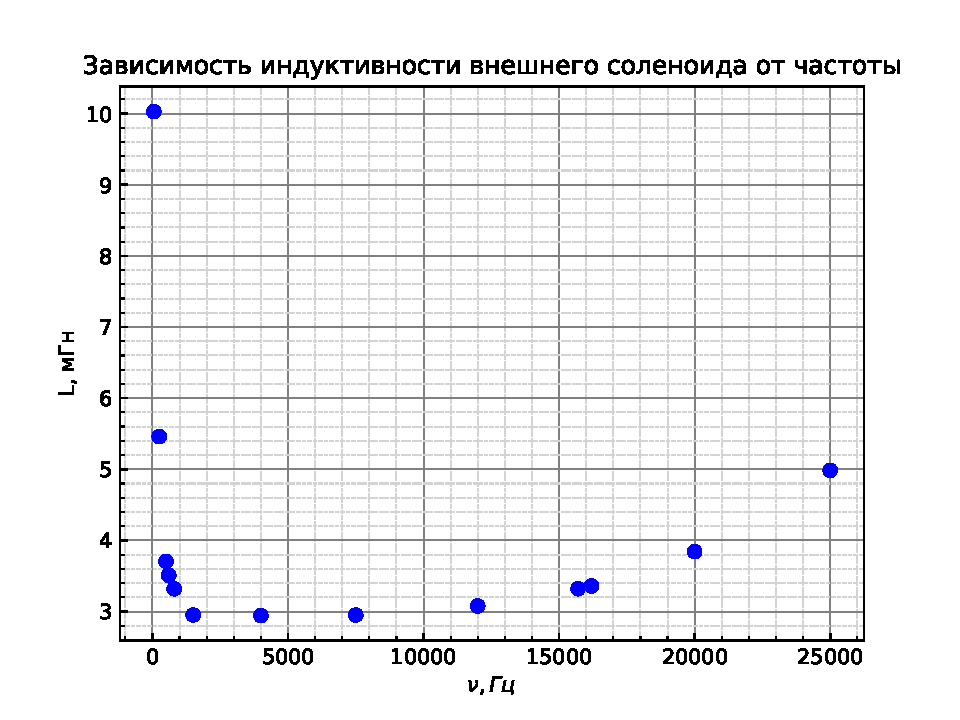
\includegraphics[width = \textwidth]{L(nu).pdf}
		\caption{График зависимости $L(\nu)$}
        \label{the inductance depends on frequency}
	\end{figure}
	
	Полученные максимальные и минимальные значения: $L_{min} = 2,94$ мГн, $L_{max} = 10,28$ мГн.

    Построим график зависимости ($L_{max} - L$)/($L - L_{min}$) от $\nu^2$ и аппроксимируем его прямой, проходящей через начало координат. По углу наклона прямой определим проводимость материала (согласно формуле (\ref{L(nu^2)})).
    
	\begin{equation*}
		\frac{L_{\max} - L}{L - L_{\min}} = \pi ^2 a^2 h^2 {\mu_0}^2 \sigma^2 \nu^2
	\end{equation*}
	
	Тогда коэффициент наклона  коэффициент наклона графика
	\[k = (\pi ah\mu_0 \sigma)^2 \ \rightarrow \sigma = \frac{\sqrt{k}}{\pi ah \mu_0}\]
	
	Подставляя полученные значения, получаем:
	
	\begin{equation}
		\sigma = (4,17 \pm 0,17) \cdot 10^7  \ \frac{\text{См}}{\text{м}}
	\end{equation}
	
	\begin{figure}[h!]
		\centering
		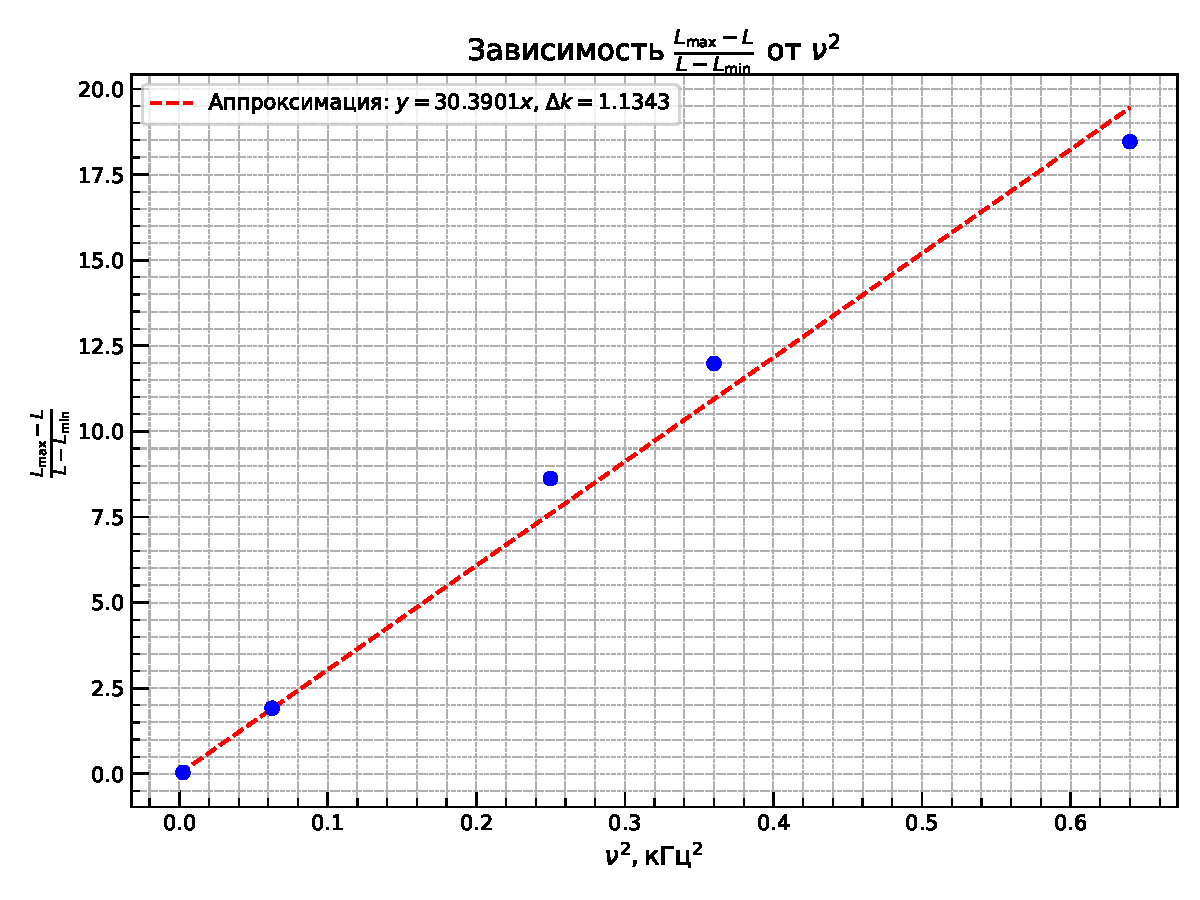
\includegraphics[width=\textwidth]{L(nu^2).pdf}
		\caption{График зависимости $\frac{L_{\max} - L}{L - L_{\min}} (\nu^2)$}
	\end{figure}
	
	
	\subsection{Коэффициент ослабления поля}
	Отношение $\abs{H_1}/\abs{H_0}$ можем посчитать, использовав полученное значение $\xi_0$ при анализе амплитуд в области низких частот.
    
	Второй способ - непосредственно через минимальный и максимальный коэффициенты проводимости $\sigma$, используя формулу (\ref{The relationship between the H_1 and H_0}). На всём диапазоне исследуемых частот построим графики зависимости коэффициента ослабление поля от частоты и сравним теоретическую и экспериментальную зависимости.
	$\abs{H_1}/\abs{H_0} (\nu)$
	
	\begin{figure}[h!]
		\centering
		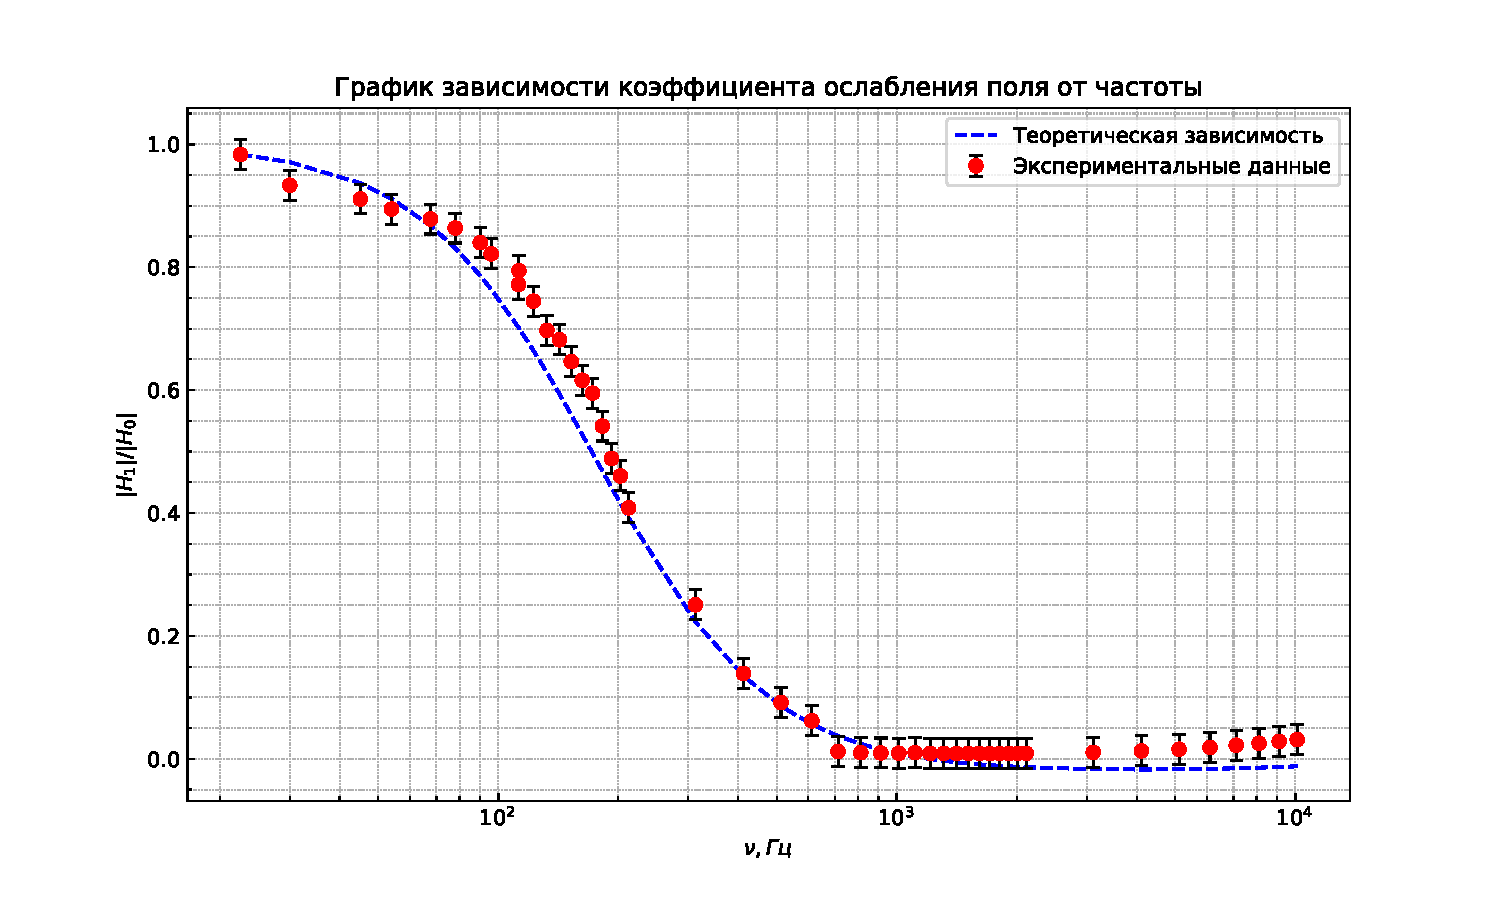
\includegraphics[width=\textwidth]{Field attenuation coeff.pdf}
		\caption{Сравнение теоретической (\ref{The relationship between the H_1 and H_0}) и экспериментальной зависимости коэффициента ослабления поля от частоты}
        \label{field parametr decrease}
	\end{figure}

    \newpage
    
	\section {Вывод}
	В данной лабораторной работе мы измеряли удельную проводимость медного образца цилиндра 4-мя при изучении скин-эффекта.
	
	\begin{table}[h!]
		\begin{center}
			\begin{tabular}{|l|c|c|c|}
				\hline
				Метод измерения & $\sigma, 10^{7} \ \frac{\text{См}}{\text{м}}$ & $\Delta\sigma, 10^{7} \ \frac{\text{См}}{\text{м}}$ & $\varepsilon_{\sigma}$\\
				\hline
				Отношение амплитуд & 5,603 & 0,014 & 0,01\%\\ \hline
				Разности фаз (низкие частоты) & 3,07 & 0,23 & 45,1\%\\ \hline
				Разности фаз (высокие частоты) & 5,05 & 0,17 & 9,6\%\\ \hline
				Индуктивность & 4,17 & 0,17 & 25,1\%\\ \hline
				
			\end{tabular}
		\end{center}
		\caption{Сравнение результатов различных методов}\label{}
	\end{table}
	
	В работе использовалась медь марки $M3$, для которой $\sigma_{\text{табл}} = 5,62\cdot10^{7} \ \frac{\text{См}}{\text{м}}$. Как мы видим, способ по отношению амплитуд самый точный, поскольку при измерении использовались фактически только измерительные приборы без осциллографа. При использовании метода измерения фаз на высоких и низких частотах существенное влияние оказывает погрешность измерения по осциллографу и размытость картинки из-за ослабления поля и сильных краевых эффектов, когда толщина скин слоя лежит на границе стенок цилиндра и наше приближение нельзя считать квазистационарным. Однако, даже на низких частотах при этом погрешность входит в $2 \sigma$, что говорит о плохой допустимости этого метода измерений.

    Индуктивность сложным образом зависит от частоты \ref{the inductance depends on frequency} и при построении линеаризованного графика при частотах $L$, приближающихся к $L_{min}$, график испытывает резкий скачок при стремлении к 0 знаменателя. Первые точки плохо характеризуют зависимость, поскольку она является асимптотической ($\Delta k = 1,13$), только относительная погрешность определения МНК составила 4 \%, при учёте погрешностей прибора, которая включает погрешность определения и выбора частоты, некоторую неисправность используемого $LCR-\text{метра}$, имеем, что метод носит только оценочный характер.  
	
	Экспериментальная и теоретическая зависимости $\frac{|H_1|}{|H_0|} (\nu)$ согласно графику (\ref{field parametr decrease}) хорошо совпадают на высоких частотах, когда глубина скин-слоя маленькая и поле сосредоточено у поверхности (с учётом пересечений с крестами погрешностей теоретической зависимости). Однако в диапазоне средне-высоких частот, во время переходного процесса, показания чуть выше предсказываемых, что опять же может быть связано с упрощением модели квазистационарности и полубесконечного идеального цилиндра.

    


\end{document}